% Appendix: additional qualitative results (user 2026-11-02: no page limit, up to ~18 pages).
% Figures: figures/src/make_qual_figs.py (scenes chosen in figures/qualbank/selection.yaml from
% figures/source_data/qualbank/deliver_candidates.csv, built over all 1897 test images by figures/qualbank/qualbank.py)
\appendices
\section{Additional Qualitative Results}
\label{app:qual}
Figs.~\ref{fig:supp1}--\ref{fig:supp3} show the second- and third-ranked scenes of every condition under the rule of Fig.~\ref{fig:adverse} (largest per-image mIoU gap between our model and the best of the other three models; no two scenes of a condition from the same sequence). Together with Fig.~\ref{fig:adverse} they are the 18 highest-ranked scenes of the five weather and lighting conditions and under-exposure. The candidates are computed over all 1897 test images of every model, so any scene can be replaced without new inference.

The rule picks scenes in our favour by construction. To show what an ordinary scene looks like, Fig.~\ref{fig:typical} takes, for each condition, the scene whose gap is closest to that condition's median gap. Note that the median gap is slightly negative (about $-1$ to $-2$ points in every condition): the reference is, per image, the best of three other models, so a single model rarely beats it on a typical image even when it has the highest dataset mIoU.

The DELIVER test split also contains sequences with a built-in sensor fault (over-exposure, motion blur, LiDAR jitter, low-resolution events). Figs.~\ref{fig:cases} and~\ref{fig:cases_reverse} show the scene of each fault with the largest gap in our favour and against us; the second column is the affected sensor. Fig.~\ref{fig:thin_scenes} ranks scenes by the gain on one thin class instead of the image mIoU. \todo{MUSES and MCubeS scenes; DELIVER missing-sensor scenes}

\begin{figure*}[p]
\centering
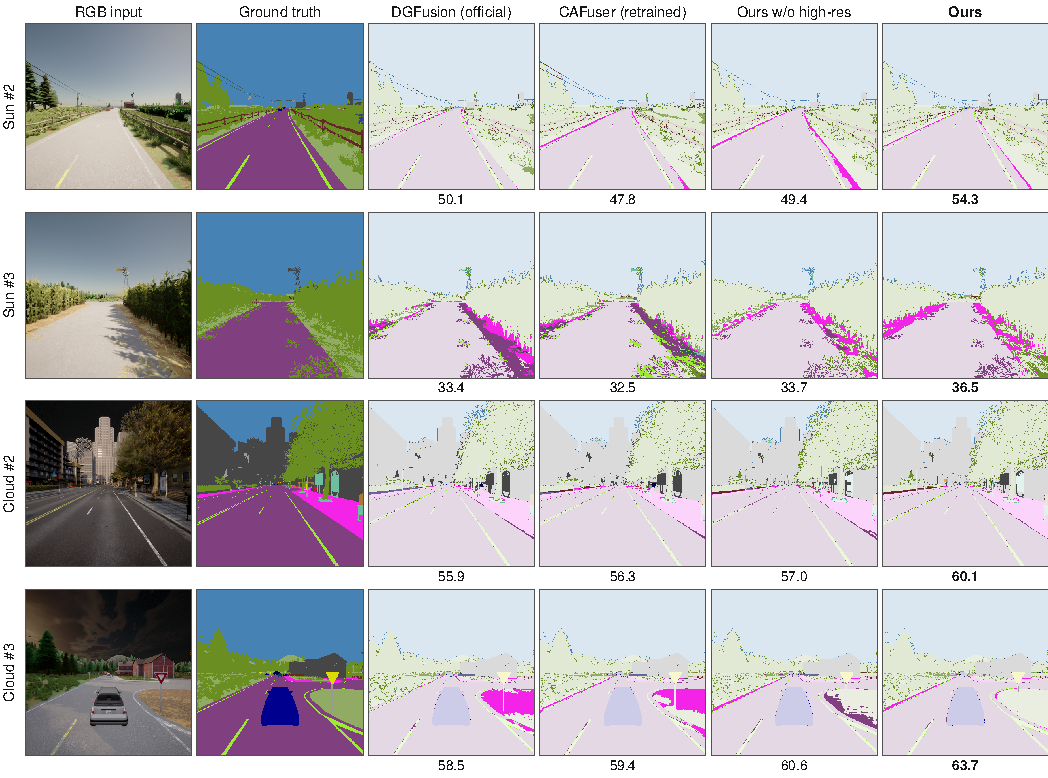
\includegraphics[width=\textwidth]{figures/fig_supp_deliver_1.pdf}\\[3pt]
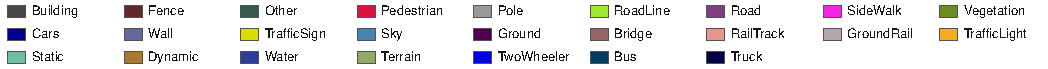
\includegraphics[width=\textwidth]{figures/fig_class_legend_deliver.pdf}
\caption{Additional qualitative results on the DELIVER test set for sun and cloud: the second- and third-ranked scenes under the selection rule of Fig.~\ref{fig:adverse}. Faded pixels agree with the ground truth; numbers give per-image mIoU (\%).}
\label{fig:supp1}
\end{figure*}

\begin{figure*}[p]
\centering
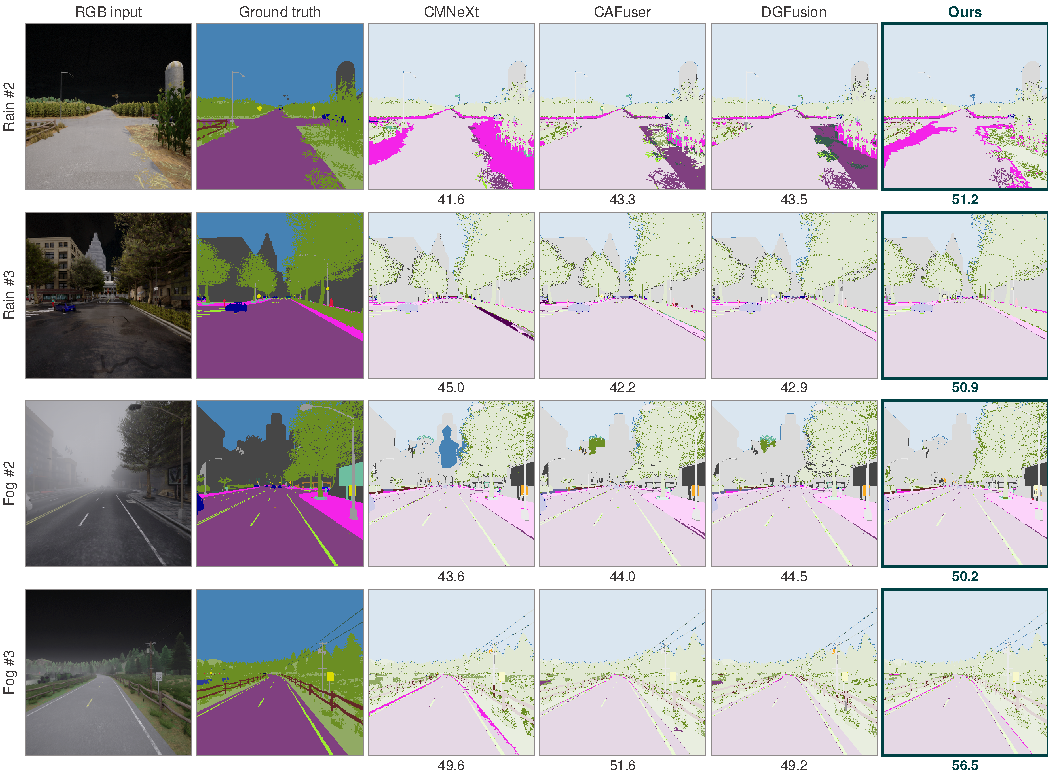
\includegraphics[width=\textwidth]{figures/fig_supp_deliver_2.pdf}\\[3pt]
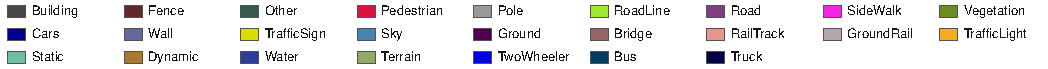
\includegraphics[width=\textwidth]{figures/fig_class_legend_deliver.pdf}
\caption{Additional qualitative results for rain and fog. Display as in Fig.~\ref{fig:supp1}.}
\label{fig:supp2}
\end{figure*}

\begin{figure*}[p]
\centering
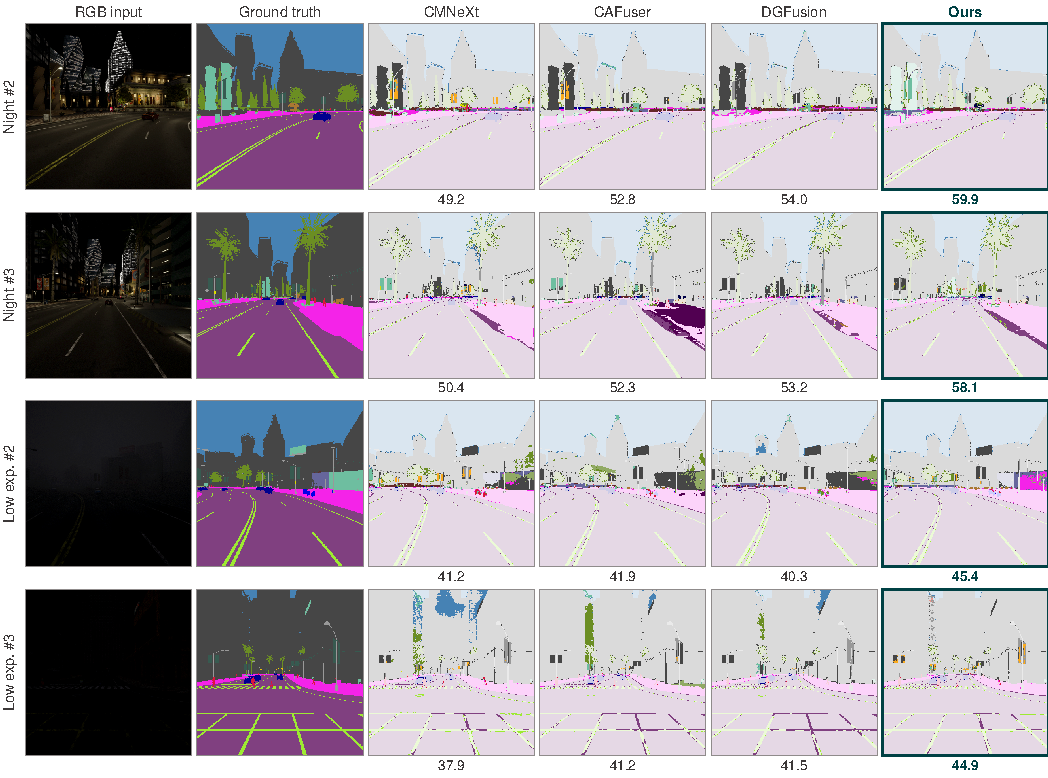
\includegraphics[width=\textwidth]{figures/fig_supp_deliver_3.pdf}\\[3pt]
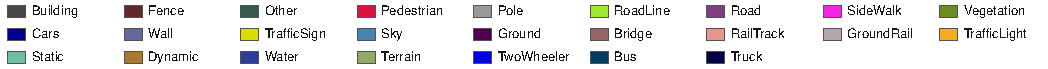
\includegraphics[width=\textwidth]{figures/fig_class_legend_deliver.pdf}
\caption{Additional qualitative results for night and low exposure. Display as in Fig.~\ref{fig:supp1}.}
\label{fig:supp3}
\end{figure*}

\begin{figure*}[p]
\centering
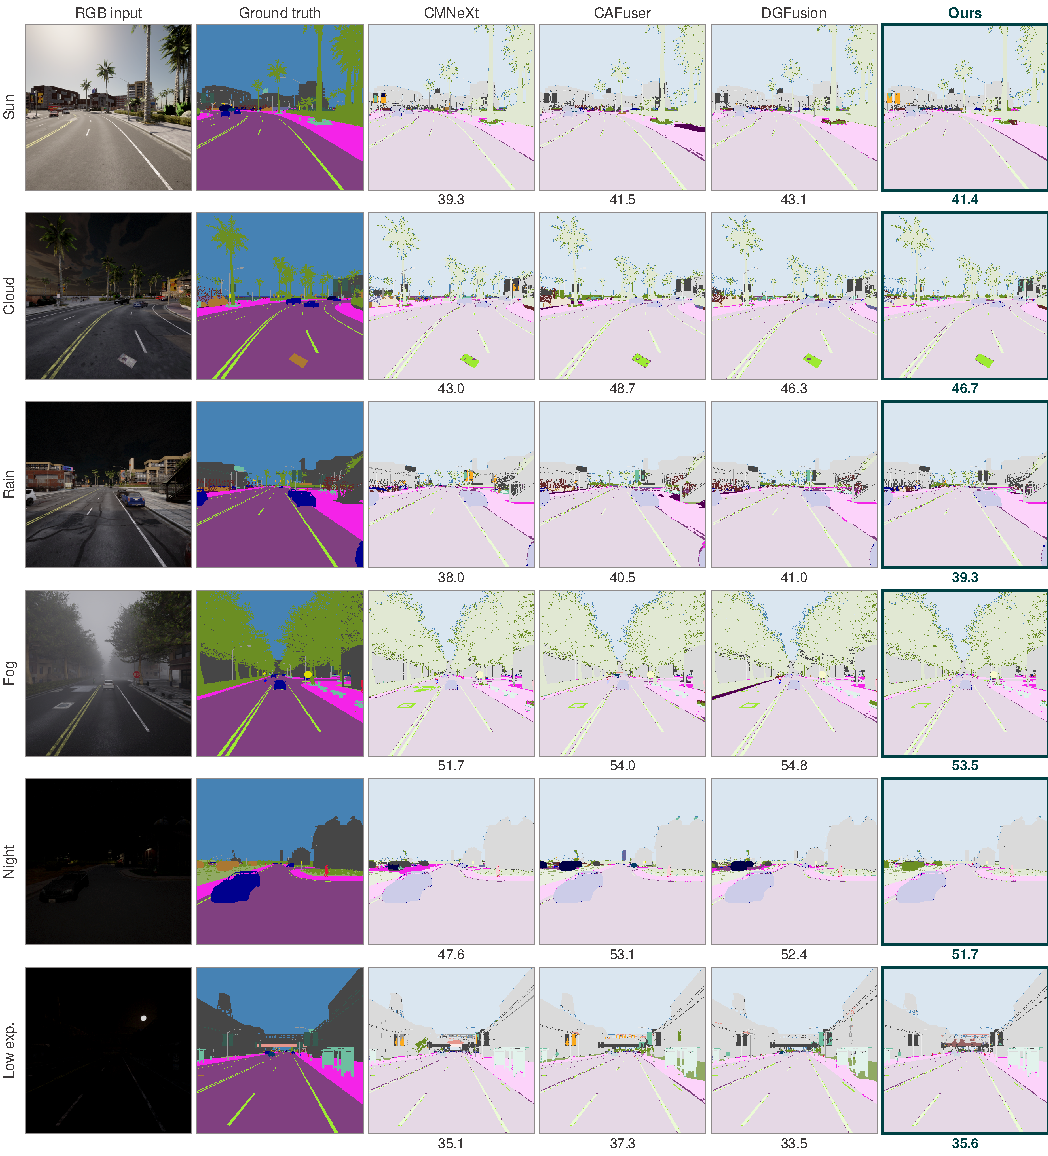
\includegraphics[width=\textwidth]{figures/fig_typical_deliver.pdf}\\[3pt]
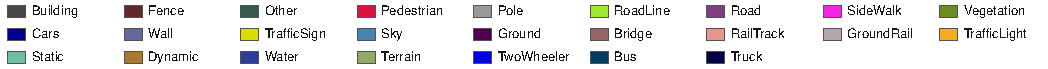
\includegraphics[width=\textwidth]{figures/fig_class_legend_deliver.pdf}
\caption{Typical scenes on the DELIVER test set: for each condition, the image whose per-image mIoU gap between ours and the best other method is closest to the median gap. Display as in Fig.~\ref{fig:supp1}.}
\label{fig:typical}
\end{figure*}

\begin{figure*}[p]
\centering
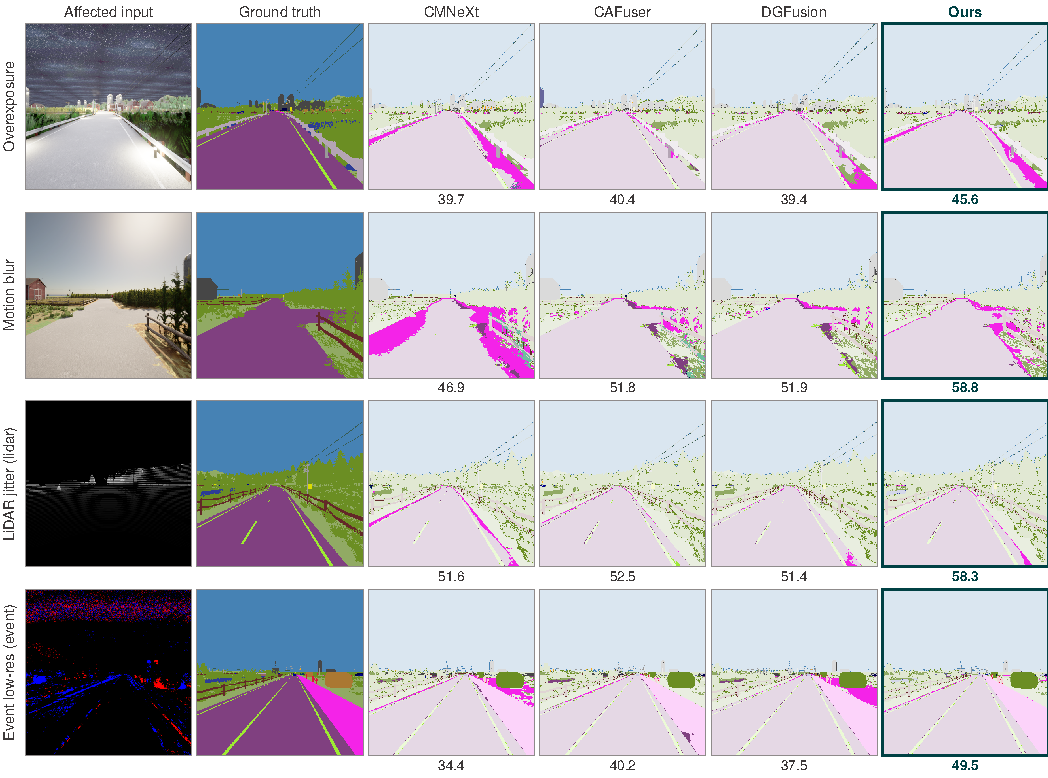
\includegraphics[width=\textwidth]{figures/fig_cases_deliver.pdf}\\[3pt]
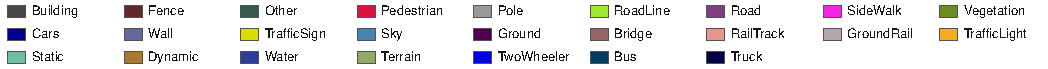
\includegraphics[width=\textwidth]{figures/fig_class_legend_deliver.pdf}
\caption{Qualitative results on DELIVER test sequences with a built-in sensor fault: for each fault, the scene with the largest per-image mIoU gap in favor of ours. The second column shows the affected sensor (RGB for exposure and blur, LiDAR, or event). Display as in Fig.~\ref{fig:supp1}.}
\label{fig:cases}
\end{figure*}

\begin{figure*}[p]
\centering
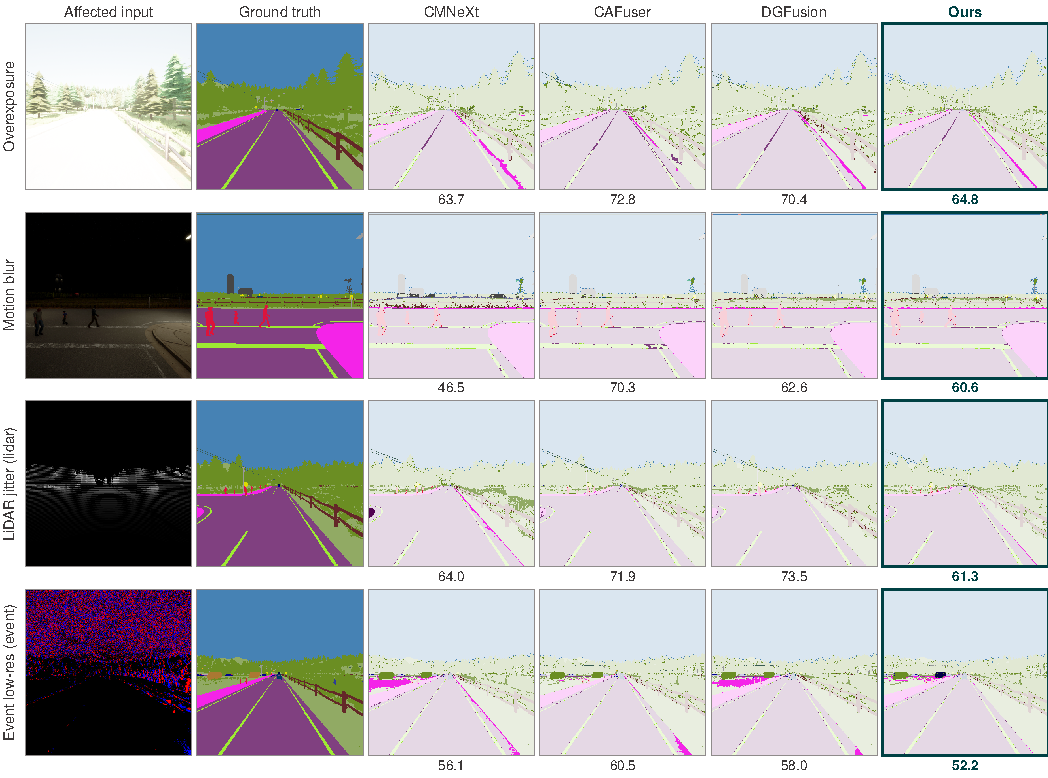
\includegraphics[width=\textwidth]{figures/fig_cases_reverse_deliver.pdf}\\[3pt]
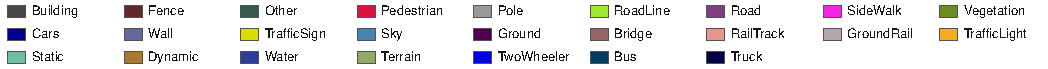
\includegraphics[width=\textwidth]{figures/fig_class_legend_deliver.pdf}
\caption{Failure cases on DELIVER test sequences with a built-in sensor fault: for each fault, the scene where another method most exceeds ours. Display as in Fig.~\ref{fig:cases}.}
\label{fig:cases_reverse}
\end{figure*}

\begin{figure*}[p]
\centering
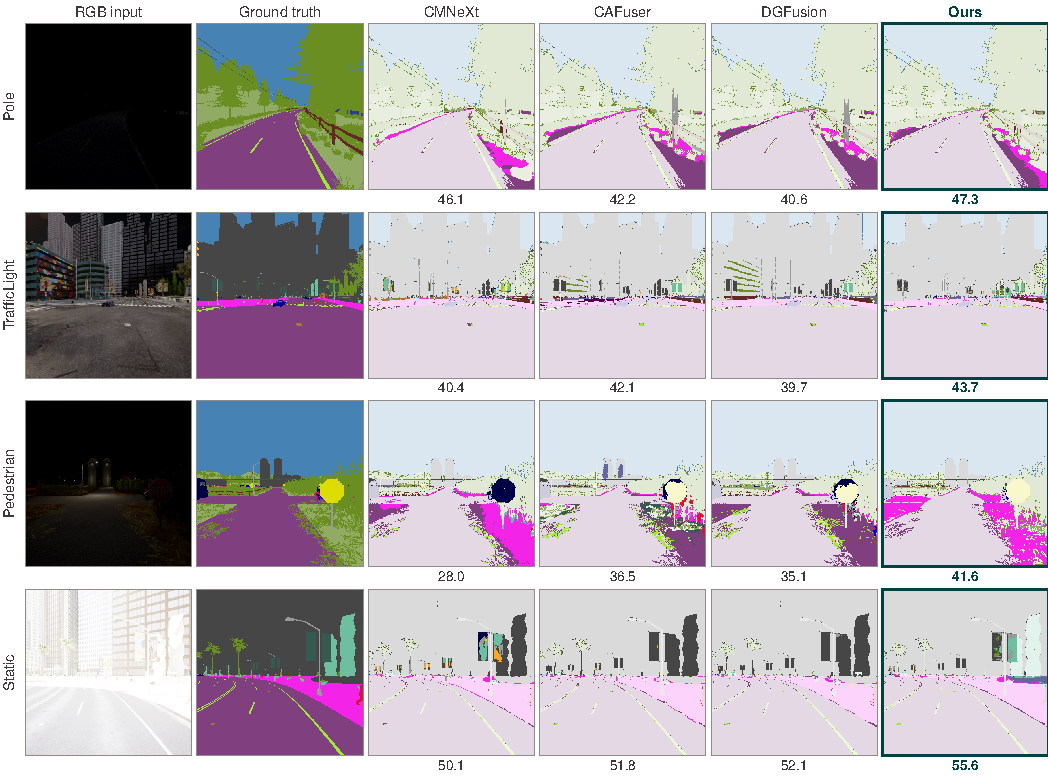
\includegraphics[width=\textwidth]{figures/fig_thin_deliver.pdf}\\[3pt]
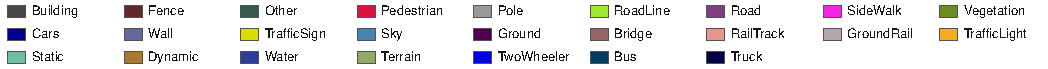
\includegraphics[width=\textwidth]{figures/fig_class_legend_deliver.pdf}
\caption{Thin classes on the DELIVER test set: for each of Pole, TrafficLight, Pedestrian, and Static, the image where the class IoU of ours most exceeds that of the best other method (at least 400 ground-truth pixels of the class). Numbers give per-image mIoU over all classes (\%).}
\label{fig:thin_scenes}
\end{figure*}
